

\chapter{Particle In cell} % Write in your own chapter title
\label{Chapter3}
\lhead{Chapter 3. \emph{A Chapter}} % Write in your own chapter title to set the page header

Simulations are used to mimic the physical world by solving the appropriate laws of physics and have a wide range of applications across all disciplines of science. Simulations provide a third tool alongisde theory and experiments to explain physical phenomena. Deep insight into the physics of plasmas has been gained by using computer simulations most notably the use of gyrokinetic codes to model the instabilities of plasmas in a tokamak. As computer power continues to increase so does the capability of computer simulations to explore the natural world.

Various techniques have been developed to simulate plasmas and they mostly fall into one of three categories. Particle-In-Cell (PIC) codes which follow the trajectories of individual particles in the plasma, Magneto-Hydrodynamics (MHD) models that treat the plasma components as fluids and Hybrid models that use a combination of MHD and PIC techniques to model the plasma. Each method has certain advantages and disadvantages that determine where its use is applicable. These will be discussed below.

PIC codes are considered to be the most fundamental way to model a plasma. Individual electrons and ions are tracked as they move across a spatial domain responding to self consistent electric and magnetic fields generated by the electric charge of the particles. Particle positions and velocities are updated at each time step by calculating the force acting on each particle and solving Newtons equations of motion. In order to reduce statistical noise in the simulations large numbers of particles must be followed and there are certain stability criteria that must be met. As a result PIC simulations are computer intensive, the simulations take a long time to run but can also provide the most insight.

Fluid codes ease the computational burden by treating the ions and electrons as separate fluids. The fluid equations are then solved to obtain macroscopic quantities of the plasma such as its density. The fluid equations require closure conditions that must be approximated. These assumptions hinder the accuracy of fluid modelling and may prevent all of the relevant physics from being captured in the model. Hybrid models exist that combine aspects of fluid and PIC codes. A common implementation of this technique is to treat the electrons as a fluid while modelling the ions kinetically. This reduces the number of particles that have to be followed and minimises the slowdown from satisfying certain stability criteria.


It is not possible to simulate a Langmuir probe without capturing the physics of the sheath. The plasma sheath cannot be correctly modelled by fluid codes as the particle distributions inside the sheath are far from being in equilibrium. The exact position of the sheath boundary is not well defined either. PIC codes on the other hand make no assumptions about the distribution of the particles and are capable of capturing all of the relevant physics on small enough time-scales. The rest of this chapter will proceed to describe the general PIC method before moving on to describe each step of the algorithm in more detail. 
%These simulations support theoretical and experimental studies and are used to understand experimental data. It is far easier to insert diagnostics into a computer simulation than it is to implement them into an experiment, a simulation therefore provides information that experiments are not able to do such as following the exact trajectory of a particle as it moves through space and time or keeping a track of its individual kinetic and potential energy. 



\subsection{General Method} 

PIC codes were first used in 1955 for the simulation of hydrodynamic problems and have been used since the 1950's for the simulation of plasma systems \cite{Harlow}. They are conceptually simple and can be implemented from first principles without the need for approximate equations of state. Their relative ease of implementation as well using physics models based on first principles makes PIC codes a popular choice for kinetic modelling. PIC simulations track the position and velocity of all the particles in the simulation domain. Particles are given an initial position and velocity which is then updated at each time step based on the forces acting on the particle. For simplicity a one dimensional model will be considered but PIC codes are used to model fully three dimensional problems. In the one dimensional case particles are free to move over a continuous domain of length $L$ and can take any position between 0 and $L$. Plasma particles interact with each other via direct collisions and electrostatic forces. To calculate the forces acting on each particle due to every other particle present in the system would be far too computationally expensive when there are large numbers of particles present such as the case in plasma simulations. This technique is commonly employed in condensed matter studies and is known as the particle-particle (PP) method. To make the simulations computationally  feasible PIC codes discretise the domain into a grid as shown below.
\begin{figure}[H]
\centering
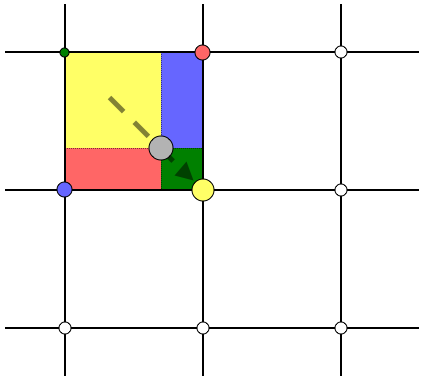
\includegraphics[width=0.8\textwidth]{grid}
\caption{A representation of a two dimensional grid. The particle (grey circle) moves through the domain and deposits charge on the grid points. The area of the rectangle is proportional to the amount of charge deposited at each grid point.\cite{grid}}
\label{fig:Leapfrog}
\end{figure}

The grid is a mathematical construct that makes it possible to solve differential equations such as Newtons equations of motion and Poissons equation for the electrostatic potential. It also allows particles to interact with each other via a charge density rather than having to calculate the force between every pair of particles and so greatly reduces the run time of simulations. Splitting a physical, continuous domain  up into grid cells does have implications which need to be considered in order to ensure the simulation can still produce physically accurate results. The consequences of introducing a grid on to the domain and how this can still accurately represent a plasma will be discussed in this report.

A PIC simulation follows an algorithm that starts with weighting the charge density of particles on to each grid point, typically particles will contribute charge only to the grid points closest to them. Different weighting schemes are possible and will be discussed. Once the charge density has been calculated it is then used to work out the electric potential by solving Poisson's equation. Again the potential is only solved at each grid point. Potential values are now used to calculate electric field values at the grid points which are then interpolated back to the particles, typically using the same weighting as for charge density so that new particle velocities and positions can be determined. Once the particles have been moved, the PIC algorithm is complete, time is advanced by one time step and the whole cycle repeats with a new density being calculated based on the new positions of the particles. This cycle will carry on until a certain time has been reached or steady-state has been obtained. PIC simulations are restricted by the size of the grid cells and the value of the time step as will be explained in more detail.
\begin{figure}[H]
\centering
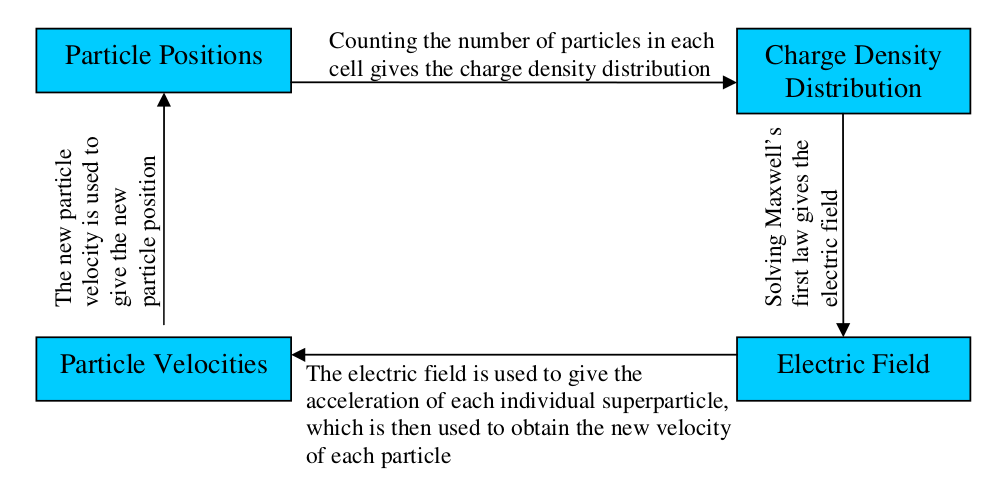
\includegraphics[width=0.8\textwidth]{piccycle}
\caption{A flow chart of the PIC algorithm \cite{loop}}
\label{fig:Leapfrog}
\end{figure}


%"A proper understanding of the sheath phenomena is also an important prerequisite for obtaining boundary conditions for fluid codes simulating tokamaks."
\subsubsection{Calculating the Density}
As discussed before particles are free to take any position along the domain and their positions determine the amount of charge they contribute to the grid points nearest them. Different weighting schemes can be used, some more accurate(less noisy) than others but at the expense of longer computation time. Weighting is the name given to how the charge density on the discrete grid points is distributed and also how the force exerted on the particles from the grid points is then calculated. The simplest weighting method is the Nearest Grid Point (NGP) scheme. This is a zero order weighting method in which the entirety of the particles charge is assigned to the grid point which it is closest to. Any particles within half a cell of the grid point are assigned to that grid point. Let the cell width be $\Delta x$, $x$ the distance from the grid point and $W(X)$ denote the weighting at grid point $X$. In the NGP scheme 

\be
    W(x)=
    \begin{cases}
      1, & \text{if}\ x \leq \frac{\Delta x }{2}   \\
      0, & \text{otherwise}
    \end{cases}
\ee

This is a computationally fast weighting method as it only requires one grid point look up per particle. As a particle moves away from a grid point and into the region of another grid point the grid density at that grid point jumps up to have a value of one and the grid point it just left falls down to 0. This gives the particle an effective shape, in this case rectangular. The particle also has a finite size of width $\Delta x$. Finite sized particles are a direct result of weighting particles on to the grid. The weighting method determines the effective size and shape of the particle as viewed by grid. Due to the large jumps to grid values caused by the movement of particles from one grid point to the next, the NGP weighting method is a large source of noise in the density and field calculations. A less noisy method is desired. 

\begin{figure}[H]
\centering
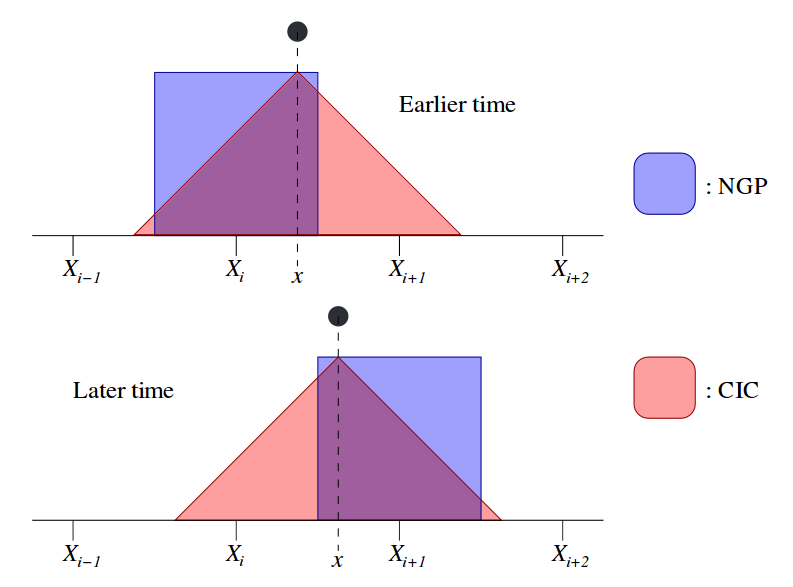
\includegraphics[width=0.8\textwidth]{particleshape}
\caption{The effective shape of a particle at position x as seen by the grid.\cite{shape}}
\label{fig:shape}
\end{figure}
First order weighting also known as the Cloud In Cell (CIC) method smooths the density and field fluctuations compared to NGP but is more computationally expensive as it requires two grid point look-ups for each particle. In this method each particle contributes charge to its nearest two grid points. The first step calculates the offset of the particle from the closest grid point to its left. 
\be
offset = x_i - X_j 
\ee 
where $x_i$ is the particles position and $X_j$ the grid point. $x_i > X_j$ always. The charge assigned to the $J^{th}$ grid point is then 
\be 
q_j = q_c \left(1 - offset\right)
\ee 
where $q_c$ is the charge of the particle. 
The charge assigned to the J+1 cell is 
\be 
q_{j+1} = q_c \left(offset\right)
\ee 
This results in a much smoother contribution to the density as the particle moves through the grid. The weighting puts the fraction of the clouds charge which is in the $J^{th}$ cell to the $X_J$ grid point and the rest of it goes to the $X_{J+1}$ grid point. This  gives the particle a triangular shape, so the particle is effectively a triangular cloud of uniform charge centred at $x_i$ with a width of $2\Delta x$ as it is able to influence a grid point from both sides of it. 

Higher order weighting methods do exist such as quadratic and cubic splines, that are second order and third order accurate respectively. These schemes further smooth the non-physical noise at the expense of more computation time by increasing the number of grid points that a particle contributes its charge to. This does lead to problems at the edge of the boundary where there are insufficient neighbouring grid points. It is unlikely that the NGP is in use in any of todays PIC codes due to the noise levels caused by interpolation but CIC is adequate for a lot of codes.

Use this for picutre %http://porl2.tripod.com/sitebuildercontent/sitebuilderfiles/mphysproject.pdf
\subsubsection{Calculating the Potential}
The potential can now be calculated from the known charge density at every grid point by solving Poisson's equation \eqref{eq:poisson}. This can be solved numerically by a computer using the Finite Difference Method (FDM). FDM solves differential equations via the discretisation of its derivatives. The first step is to carry out a Taylor series expansion of the potential, first in the forward direction.
\be
\psi(x+\Delta x) = \psi(x) + \Delta x \frac{\partial \psi}{\partial x} + \frac{{(\Delta x)}^2}{2}\frac{{\partial}^2\psi}{\partial x^2} + ...
\label{eq:forward}
\ee
The same procedure can be applied in the backwards direction 
\be
\psi(x-\Delta x) = \psi(x) - \Delta x \frac{\partial \psi}{\partial x} + \frac{{(\Delta x)}^2}{2}\frac{{\partial}^2\psi}{\partial x^2} + ...
\label{eq:backward}
\ee
These two equations can be used to give an approximate value for the second derivative of potential. Adding \eqref{eq:forward} and \eqref{eq:backward} with some rearranging gives 
\be 
\frac{{\partial}^2\psi}{\partial x^2} = \frac{\psi(x+\Delta x) -2\psi(x) + \psi(x-\Delta x)}{{(\Delta x)}^2}
\label{eq:phisolver}
\ee 
In FDM the solution to the equation is only known at the grid points, the potential is no longer a continuous function. Combining the forward difference and backward difference solution like this is known as central differencing and is second order accurate. For clarity we rewrite \eqref{eq:phisolver} with labels based on the grid number $j$. 
\be 
\frac{{\partial}^2\psi}{\partial x^2} = \frac{\psi_{j+1} -2\psi_{j} + \psi_{j-1}}{{(\Delta x)}^2} = -\frac{\rho_j}{\epsilon_0}
\label{eq:phisolver1}
\ee 

The value of $\psi$ at grid point j, ($\psi_j$),  depends on the value of $\psi$ at the two grid points either side of it $(\psi_{j-1}$ and $\psi_{j+1})$, so the grid points are coupled together. In order to find the value of $\psi_j$ at $N$ different grid points requires the solution of $N$ coupled linear equations. 


These coupled equations can be expressed in matrix form. 
\be
\begin{pmatrix}
  B_{1} & C_{1}  \\
  A_{2} & B_{2} & C_2 \\
        & A_3  & B_3 & C_3   \\
        & & \ddots & \ddots & \ddots \\
        & & &  A_N & B_N
\end{pmatrix}
\begin{pmatrix} 
 \psi_1  \\ 
 \psi_2  \\ 
 \psi_3  \\ 
 \vdots  \\
 \psi_N
\end{pmatrix}
= 
\begin{pmatrix} 
 \rho_1  \\ 
 \rho_2  \\ 
 \rho_3  \\ 
 \vdots  \\
 \rho_N
\end{pmatrix}
\ee
Where $A=1, B=-2$ and $C=1$. A matrix like this with non-zero elements only on the diagonal and one place either side of it is known as a tri-diagonal matrix.  The value of $\rho$ at each grid point is known as it was calculated in the previous step of the PIC algorithm. This matrix equation must now be solved in order to obtain the potential at each grid point. Plenty of tri-diagonal matrix solvers exist including the tridag solver found in Numerical Recipes\cite{NumericalRecipes}. Before this can be done the boundary conditions must be supplied. The first and last grid points only have one neighbouring grid point and so the previous equation no longer holds. Two common choices for boundary conditions exist, Dirichlet boundary conditions where $\psi_1$ and $\psi_N$ are set to a fixed value or Neumann boundary conditions where the gradient of the potential is fixed at the boundary. 
The implementation of Dirichlet boundary conditions is simple, $B_1$ and $B_N$ are set equal to one and $\psi_1$ and $\psi_N$ are then given the desired potential boundary values $\alpha $ and $\beta$  respectively. The first and last matrix equations then read
\be 
1.\psi_1 + 0.\psi_2 = \alpha 
\ee 
\be 
0.\psi_{N-1} + 1.\psi_N = \beta 
\ee 

Neumann boundary conditions involve fixing the gradient of the potential(i.e. the electric field) at the edge of the domain. This could be implemented by setting $B_1  = -\frac{1}{\Delta x}$, $C_1 = \frac{1}{\Delta x}$ and $\rho_1$ = $\alpha$. Thus giving the first line in the matrix equation as 
\be 
\frac{\psi_2 - \psi_1}{\Delta x} = \alpha 
\ee 

Once the boundary conditions have been supplied the tri-diagonal matrix equation can be solved.
 

\subsubsection{Calculating the Electric Field}
Once the potential is known at each grid point the electric field is easily found by calculating the gradient of the potential.
\be 
E = - \nabla \psi
\ee 
which in one dimension becomes
\be 
E = - \frac{\partial \psi}{\partial x}
\label{eq:electricfield}
\ee
This can discretised as before using the central difference method. 
\be 
E_J = - \frac{\psi_{J+1} - \psi_{J-1}}{2 \Delta x}
\ee 
Central differencing is not applicable at the boundaries due to a lack of neighbouring grid points and so either the forward or backward difference method must be used which is only accurate to first order. This provides the following two conditions to calculate the electric field at the edge of the domain.
\be
E_0 = - \frac{\psi_{J+1}-\psi_0}{\Delta x}
\ee 
\be 
E_N = - \frac{\psi_N - \psi_{N-1}}{\Delta x}
\ee
Using a first order equation at the boundaries reduces the accuracy throughout the solution to first order. Fortunately the accuracy can be improved to second order by carrying out a further Taylor expansion 
\be
\psi(x+2\Delta x) = \psi(x) + 2\Delta x \frac{\partial \psi}{\partial x} + \frac{{(2\Delta x)}^2}{2}\frac{{\partial}^2\psi}{\partial x^2} + ...
\label{eq:forward2}
\ee
Combining equations \eqref{eq:forward} , \eqref{eq:forward2} and \eqref{eq:electricfield} gives 
\be 
E_0 = \frac{3\psi_0 + \psi_2 - 4\psi_1}{2\Delta x}
\ee 
The exact same method in the backwards direction gives 
\be 
E_N = \frac{4\psi_{N-1} - \psi_{N-2} - 3\psi_N}{2\Delta x}
\ee
The second order boundary conditions restore second order accuracy across the domain.
\subsubsection{The Particle Mover}
The final step in the PIC cycle is to move the particles which requires calculating a new position and velocity for each particle in the simulation based on the forces acting on them. In order to do this Newtons equations of motion must be solved 
\be 
\vec{F}  = m \frac{d \vec{v}}{d t}
\ee 
\be 
\vec{v} = \frac{d \vec{x}}{d t}
\label{eq:diff2}
\ee 

Ignoring the presence of a magnetic field for now and limiting to one dimension gives the following equation of motion.
\be 
\frac{d \vec{v(x)}}{d t} = \frac{q}{m} E(x)
\label{eq:diff1}
\ee

The particles positions and velocities can be found by integrating the differential equations \eqref{eq:diff2} and \eqref{eq:diff1}. There are many ways in which these equations can be integrated, the methods vary in their complexity to implement as well as run time and accuracy. Depending on the needs of the simulator, a trade off may need to be made between fast run time and high accuracy. 

The simplest method of integration is Euler's method.
The finite difference method is used again to discretise the equations. 
\be 
v_{t+\Delta t} = v_t + \frac{dv}{dt} \Delta t + \frac{d^2v}{dt^2} {(\Delta t)}^2 + ...
\ee
\be 
x_{t+\Delta t} = x_t + \frac{dx}{dt} \Delta t + \frac{d^2x}{dt^2} {(\Delta t)}^2 + ...
\ee

In the Euler method The largest term neglected is $\propto {(\Delta t)}^2$. After taking $N$ steps where $N = \frac{total time}{\Delta t}$ the error is now proportional to $\Delta t$. For the case of charged particles moving in an electric field the equations of motion can now be written as
\be
v_{t+1} = v_t + \frac{qE}{m} \Delta t
\label{eq:accelerate}
\ee
\be 
x_{t+1} = x_t + v_t \Delta t
\label{eq:move}
\ee 
The field has been solved already in the previous step of the PIC cycle so $E$ is known. This is then used to accelerate the particle to a new velocity \eqref{eq:accelerate}. The new velocity is then used to find a new position \eqref{eq:move}. All particles are given an initial position and velocity at the start of the simulation so $x_0$ and $v_0$ are known.  The Euler method is very simple to implement and fast to run but is only first order accurate.

To demonstrate the stability of the Euler method it will now be applied to the case of a mass on a spring with equation of motion 
\be 
\frac{d^2 x}{dt^2} = -\frac{k}{m} x 
\ee
where $k$ is the Stiffness constant of the spring and $m$ is the mass of the attached object. An initial value for the position and velocity is required e.g. $v=1, x=0$.  Euler's method would approximate the equations of motion as 
\be
v_{t+1} = v_t - \frac{k}{m} x \Delta t 
\ee
\be 
x_{t+1} = x_t + v_t \Delta t
\ee
These equations can be solved multiple times to advance the system from its initial state. To check the accuracy of the Euler method the results are compared to the known analytical solution. 
\begin{figure}[H]
\centering
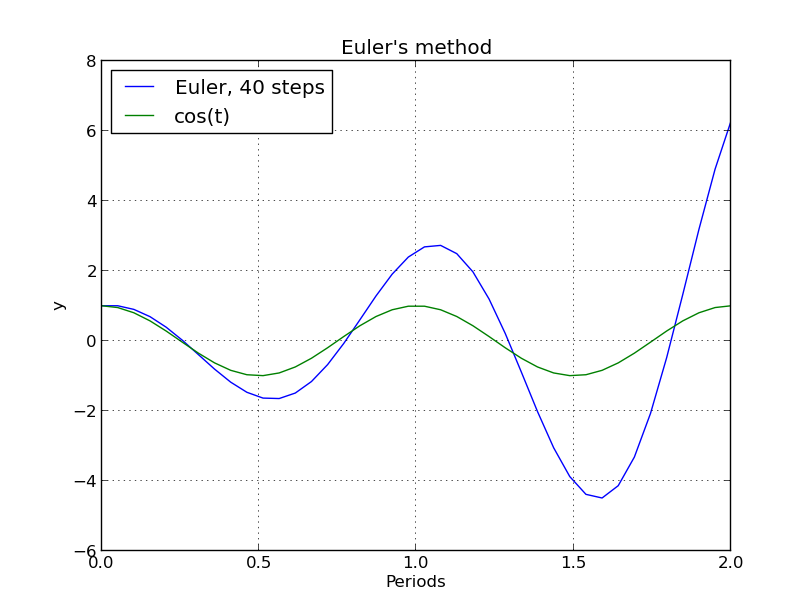
\includegraphics[width=0.8\textwidth]{Euler}
\caption{Euler solution to harmonic oscillator compared to analytical solution.}
\label{fig:E}
\end{figure}
The Euler method is unstable and quickly diverges from the analytical solution. This is no surprise based on the simplicity of the method. A more stable, higher order accurate integrator is desired for use in PIC codes.  Euler's method is described as an Explicit method as it uses the state of the system at the current time step to advance the system to its next time state. Implicit methods on the other hand use both the state of the system at the current time and the state of the system at the next time step to evolve the state of the system. An example of this is the Backwards Euler method. In this case the value of the velocity at time $t$ can be expressed as 
\be
v_t = v_{t+1 -\Delta t} = v_{t+1} - \Delta t \frac{dy}{dt}\Bigr|_{\substack{t=t+1}}
\ee
using a backwards Taylor expansion. Rearranging gives 
\be 
v_{t+1} = v_t +  \Delta t \frac{dy}{dt}\Bigr|_{\substack{t=t+1}} 
\ee 
A similar expression is found by replacing $v$ with $x$. Applying this to the case of the simple harmonic oscillator 
\be 
v_{t+1} = v_t - \Delta t\frac{k}{m} x_{t+1} 
\ee 
\be 
x_{t+1} = x_t - \Delta t\frac{k}{m} v_{t+1} 
\ee
The new value of the variable no longer depends on two known values as in the case of the Euler method but now depends on an unknown value from the next time step. It can be solved using the Newton-Raphson method. Implicit schemes are stable but more computationally expensive, this can be offset by the fact they allow for larger time steps to be taken and so can evolve a system to a desired time using less time steps than an explicit scheme. The stability of the numerical methods is not the only thing that limits the size of the time step in PIC codes, the size of the timestep is limited by the natural frequencies of the system \cite{Hockney1981}. This will be discussed more in the practical considerations section. The computational expensive and the need to use small time steps often rules out the use of implicit methods for the particle mover of PIC codes. 


Fortunately a more stable, explicit  method exists that is very similar to the Euler method and requires the same number of computations per time step but also has the advantage of being second order accurate. The Leapfrog method expands upon the Euler method. Instead of using the velocity at the beginning of the time step to advance the position it uses an average value of velocity throughout the time step. The leap-frog method involves offsetting the velocity by half a time step from the position. So the velocity of the particles is only known at half integer time steps while the positions are known at integer time steps. 
\be 
v_{t+1/2} = v_{t- 1/2} + \frac{qE_t}{m} \Delta t
\ee
\be 
x_{t+1} = x_{t} + v_{t+1/2} \Delta t
\ee 
This requires the initial velocities of the particles to be moved back half a time step at the beginning of the simulation, a "de-acceleration", in order to have time centred velocities. This just requires calculating the fields as before. This method is known as Leap-frog because in order to calculate new positions requires a leap over the known velocity. 

\begin{figure}[H]
\centering
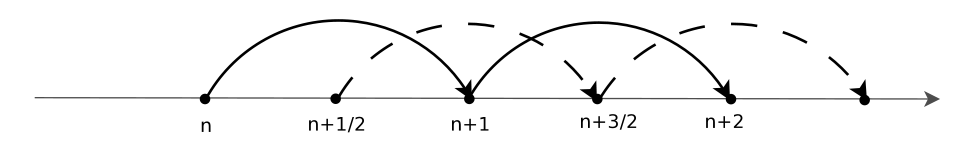
\includegraphics[width=0.8\textwidth]{Leapfrog}
\caption{A graphical representation of the Leap-Frog scheme\cite{shape}}
\label{fig:Leapfrog}
\end{figure}
Instead of using the velocity at time $t$ to move the particle from $t$ to $t+1$ like the Euler method, Leap frog uses the velocity at time $t+\frac{1}{2}$ i.e. the average velocity of the particle between those two times. This method is more accurate than Euler's method for the same computational expense. The only extra step involves pushing back the particles half a time step but this only needs to be carried out once. For this reason Leap-frog is always the preferred choice over Euler and it can be proven to be second order accurate \cite{second_order}.
This method can also be applied to the case of the mass on a spring as before and compared to the analytical solution.
\begin{figure}[H]
\centering
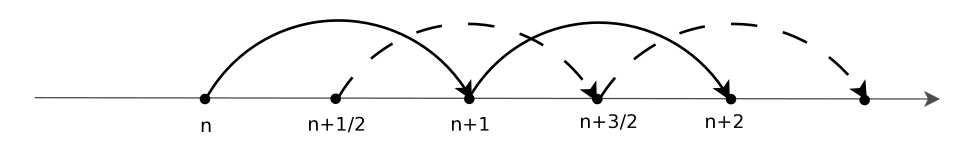
\includegraphics[width=0.8\textwidth]{leapfrog}
\caption{A comparison of the numerical solution to the problem of a mass on a spring using the leapfrog method compared to the analytical solution.}
\end{figure}
This was run with as many time steps as Euler. It is clearly more stable. As with all explicit methods there exists a critical time step size, exceeding this leads to numerical instabilities. In the case of leapfrog $w dt <2 $ where $w$ is the highest frequency in the problem, usually the electron plasma frequency. COULD PROVE THIS WITH THE HARMONIC OSCILLATOR. However as mentioned before there are other factors which force the time step to be small for PIC codes so this is not a disadvantage to the Leap Frog method.